\documentclass[a4paper,11pt]{report}
\usepackage[utf8]{inputenc}
\usepackage[T1]{fontenc}
\usepackage[italian]{babel}
\usepackage{fancyhdr}
\usepackage{indentfirst}
\usepackage{amsmath}
\usepackage{graphicx}
\usepackage{listings}
\usepackage{color}

\definecolor{mygreen}{RGB}{46,139,87}
\definecolor{myred}{RGB}{165,42,42}
\definecolor{mypurple}{RGB}{160,32,240}
\definecolor{gray}{rgb}{0.5,0.5,0.5}
\definecolor{mauve}{RGB}{255,0,255}
 
\lstdefinelanguage{myC}{%
  basicstyle=\ttfamily\footnotesize,%
  numbers=left,%
  numberstyle=\tiny\color{gray},%
  stepnumber=1,%
  numbersep=5pt,%
  backgroundcolor=\color{white},%
  showspaces=false,%
  showstringspaces=false,%
  showtabs=false,%
  frame=single,%
  rulecolor=\color{black},%
  tabsize=2,%
  captionpos=b,%
  breaklines=true,%
  breakatwhitespace=false,%
  title=\lstname,%
  keywordstyle=[1]\color{mygreen}\bfseries,%
  morekeywords=[1]{double,int,float,char,complex_t,rgb_t,plist},%
  keywordstyle=[2]\color{myred}\bfseries,%
  morekeywords=[2]{for,while,if,else,return,sizeof},%
  stringstyle=\color{mauve},%
  commentstyle=\color{blue},%
  escapeinside={\%*}{*)},%
  morecomment=[s]{/*}{*/},%
  morecomment=[l][\color{mypurple}]{\#},%
  morecomment=[l]{//},%
  morestring=[b]",%
}

\lstset{language=myC}

\title{\bfseries{\Huge{Relazioni di Laboratorio di Fisica Computazionale}}}
\author{\textit {Luca Cassia - [MAT. 728341]}}

\date{Spring 2012}

\pagestyle{fancy}\addtolength{\headwidth}{20pt}
\renewcommand{\chaptermark}[1]{\markboth{\thechapter.\ #1}{}}
\renewcommand{\sectionmark}[1]{\markright{\thesection \ #1}{}}
\cfoot{}

\rhead[\fancyplain{}{\bfseries\leftmark}]{\fancyplain{}{\bfseries\thepage}}
\lhead[\fancyplain{}{\bfseries\thepage}]{\fancyplain{}{\bfseries\rightmark}}

\begin{document}
\maketitle
\tableofcontents

\chapter{\huge Integrazione Numerica}

\section{Quadrature Gaussiane}
\section{Monte Carlo}
\section{Campionamento d'Importanza}

\chapter{\huge Algoritmo Metropolis}

\section{L'Oscillatore Armonico Quantistico}
\begin{center}
$\langle X_l X_k\rangle = 2|\langle\tilde{E}_0|\hat{x}|\tilde{E}_1\rangle|^2 exp\left(-\frac{Na}{2}(\tilde{E}_1-\tilde{E}_0)cosh\left[a\left(\frac{N}{2}-|l-k|\right)(\tilde{E}_0-\tilde{E}_1)\right]\right)$
\end{center}
\section{Azione e Termalizzazione}

Inizializzando il vettore della configurazione con numeri casuali è necessario lasciare del tempo al sistema per portarsi allo stato di equilibrio, dove, per l'ipotesi di ergodicità, tutte le configurazioni possibili sono equiprobabili. Tale processo, denominato termalizzazione, richiede di norma non più di 500 cicli di metropolis, eseguiti i quali sarà possibile estrarre le configurazioni con la giusta distribuzione di probabilità. Vi sono due modi di porre le condizioni iniziali:
\begin{itemize}
   \small
   \item[-] Azione ''fredda'' : le variabili sono inizializzate a zero.
   \item[-] Azione ''calda'' : le variabili sono inizializzate a valori diversi da zero.
\end{itemize}
\begin{figure}[h]
\centering
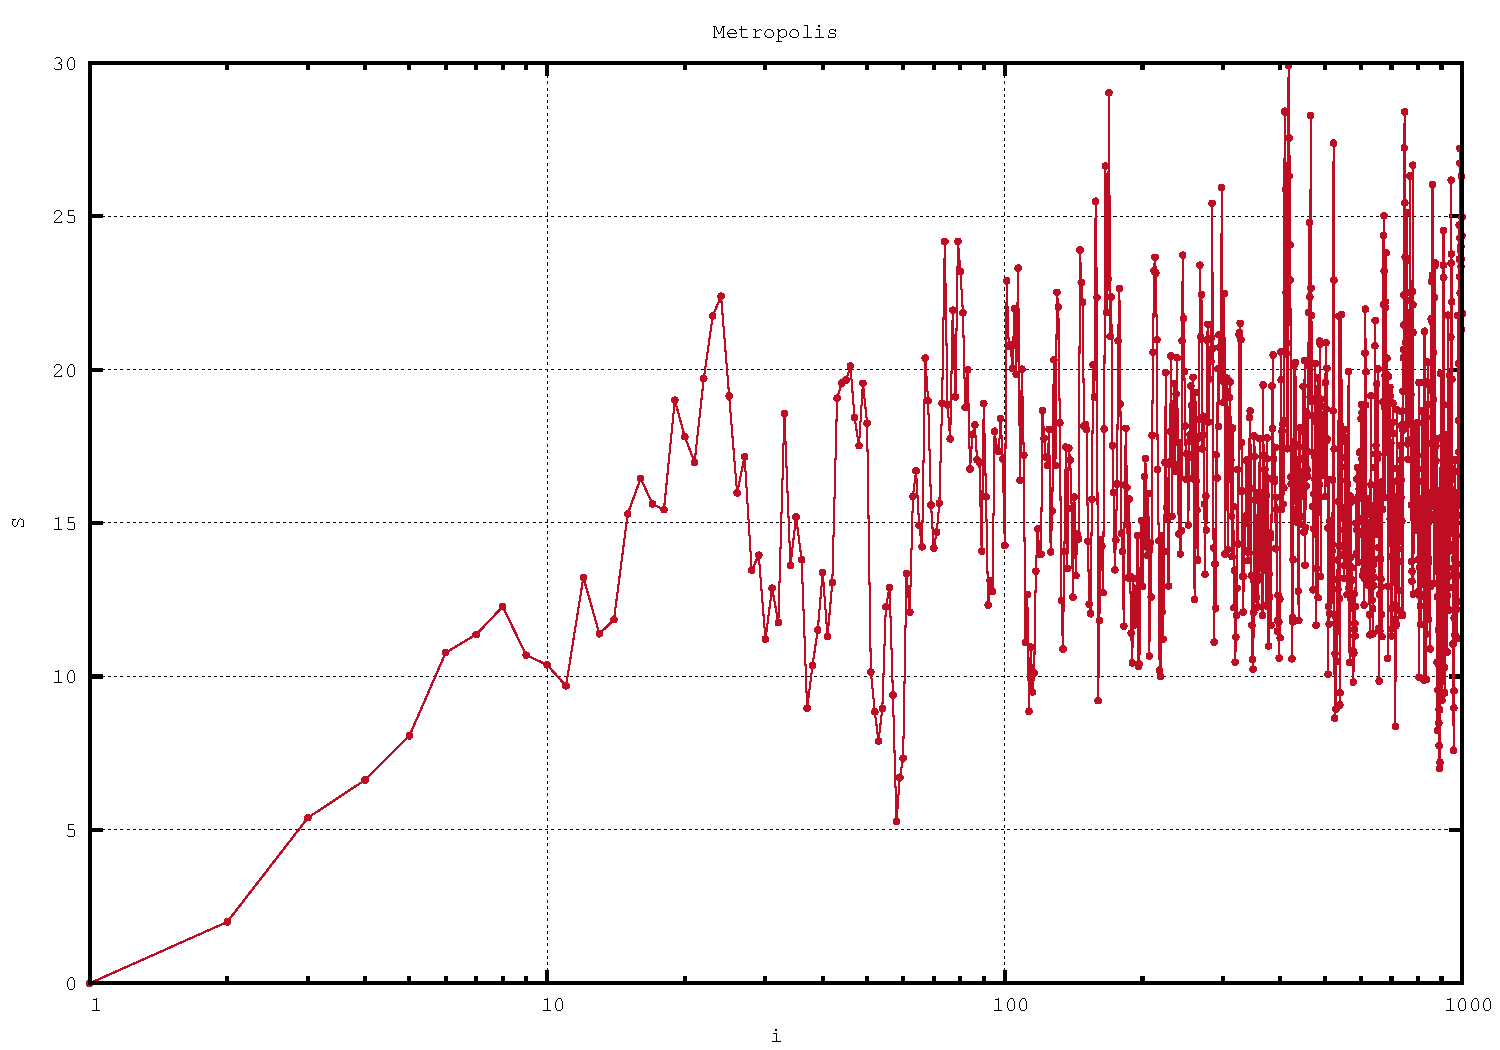
\includegraphics[width=0.5\textwidth]{action1}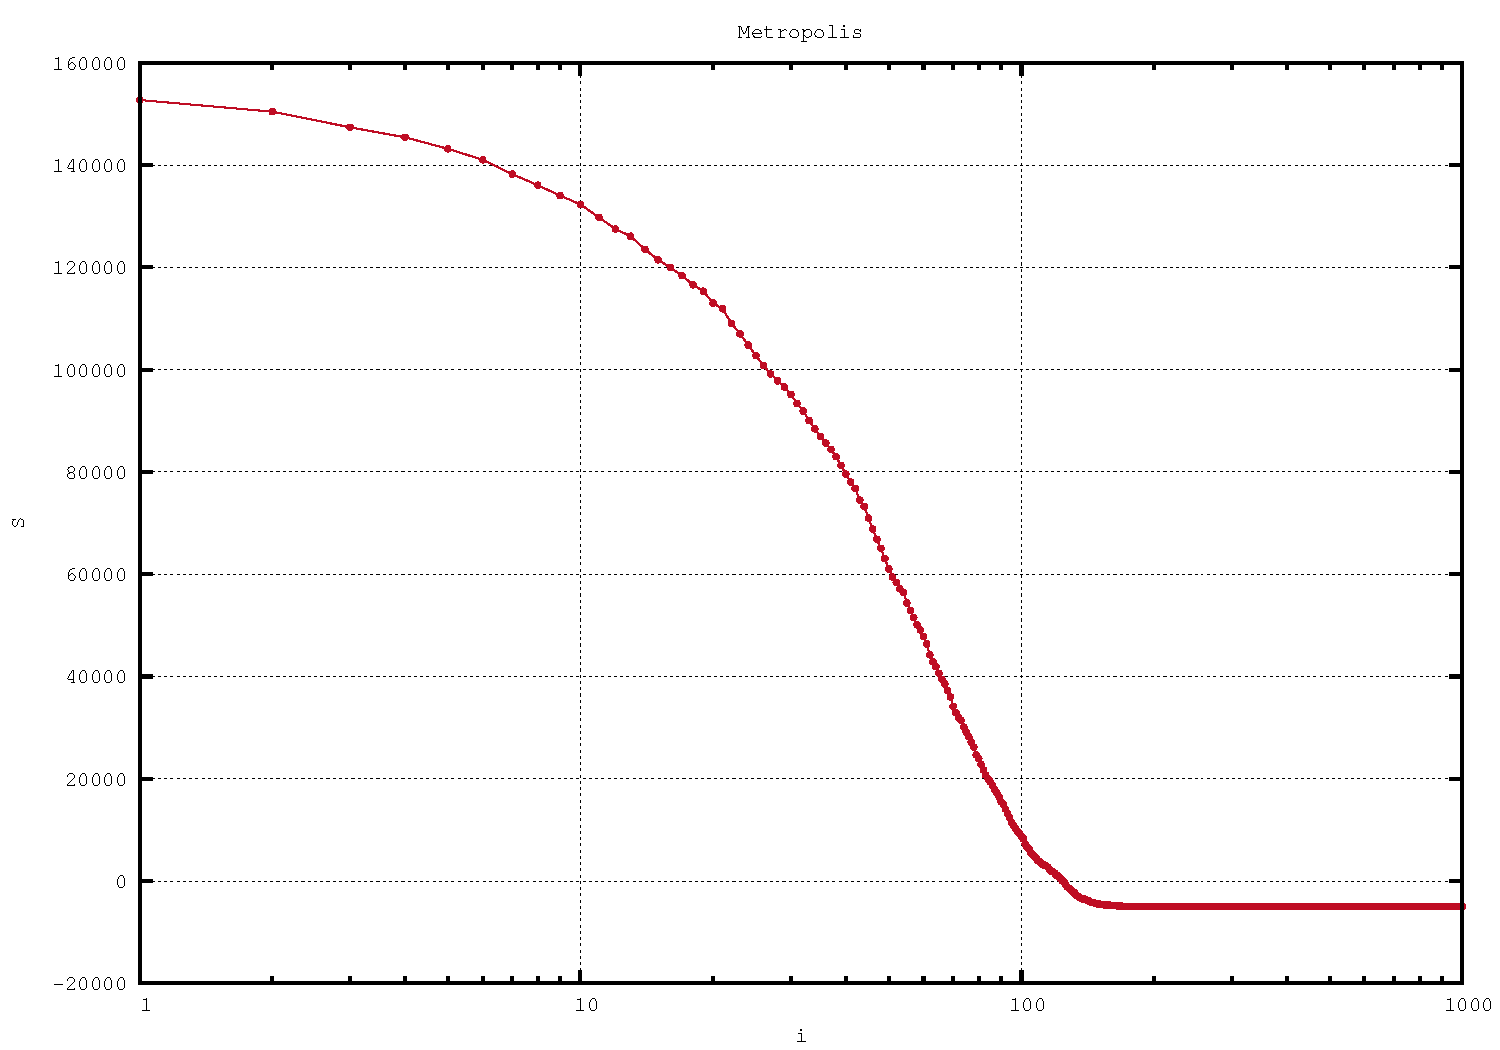
\includegraphics[width=0.5\textwidth]{action2}
\caption{Azione Fredda e Calda}
\label{fig:action}
\end{figure}
Per il calcolo dell'azione euclidea si usa la formula
\begin{center}$S = a\displaystyle\sum\limits_{i=0}^{N-1} \mathcal{L}(x_{i},x_{i+1})$\end{center}
dove
\begin{center}$\mathcal{L}(x_{i},x_{i+1}) = \frac{m}{2}\left(\frac{x_{i}-x_{i+1}}{a}\right)^{2}-\frac{1}{2}V(x_{i})-\frac{1}{2}V(x_{i+1})$\end{center}
Per calcolare il $\Delta S = S'-S$ si può tenere presente il fatto che ad ogni estrazione solo una variabile di sistema viene modificata e quindi tutti i termini delle due sommatorie che non contengono quella variabile si elidono nella differenza. Pertanto si utilizza la formula ridotta
\begin{eqnarray*}
 \Delta S_i &=& a[\mathcal{L}(x_{i-1},x'_{i})+\mathcal{L}(x'_{i},x_{i+1})-\mathcal{L}(x_{i-1},x_{i})-\mathcal{L}(x_{i},x_{i+1})]\\
   &=& M[(x_{i}-x'_{i})(x_{i+1}+x_{i-1})+(x'^2_i-x^2_i)]+V(x'_i)-V(x_i)
\end{eqnarray*}

Il codice corrispondente è
\lstinputlisting[firstline=9,lastline=28,firstnumber=9]{main/metropolis.c}
dove le variabili {\ttfamily M} e {\ttfamily W} corrispondono alla massa e alla pulsazione riscalate del fattore $a$ mentre la {\ttfamily y} argomento della funzione {\ttfamily dS()} corrisponde alla nuova variabile estratta $x'_{i}$. Si noti che le condizioni di periodicità al contorno del reticolo sono implementate attraverso l'algebra modulo N sugli indici del vettore {\ttfamily x}.

Il ciclo di termalizzazione viene eseguito all'interno del {\ttfamily main()}:
\lstinputlisting[firstline=84,lastline=89,firstnumber=84]{main/metropolis.c}
La funzione {\ttfamily metropolis()} esegue uno sweep sul vettore {\ttfamily x} delle variabili di sistema aggiornandole una alla volta con probabilità $e^{-\Delta S_i}$, e restituendo infine la variazione di azione totale {\ttfamily DS} = {\ttfamily $\sum$ ds} = $\sum^{N-1}_{i=0}\Delta S_i$.
\lstinputlisting[firstline=30,lastline=42,firstnumber=30]{main/metropolis.c}
La variabile $x'_i$ è estratta con una distribuzione piatta in un'intorno sferico di $x_i$ di raggio {\ttfamily D}.

\begin{figure}[h]
\centering
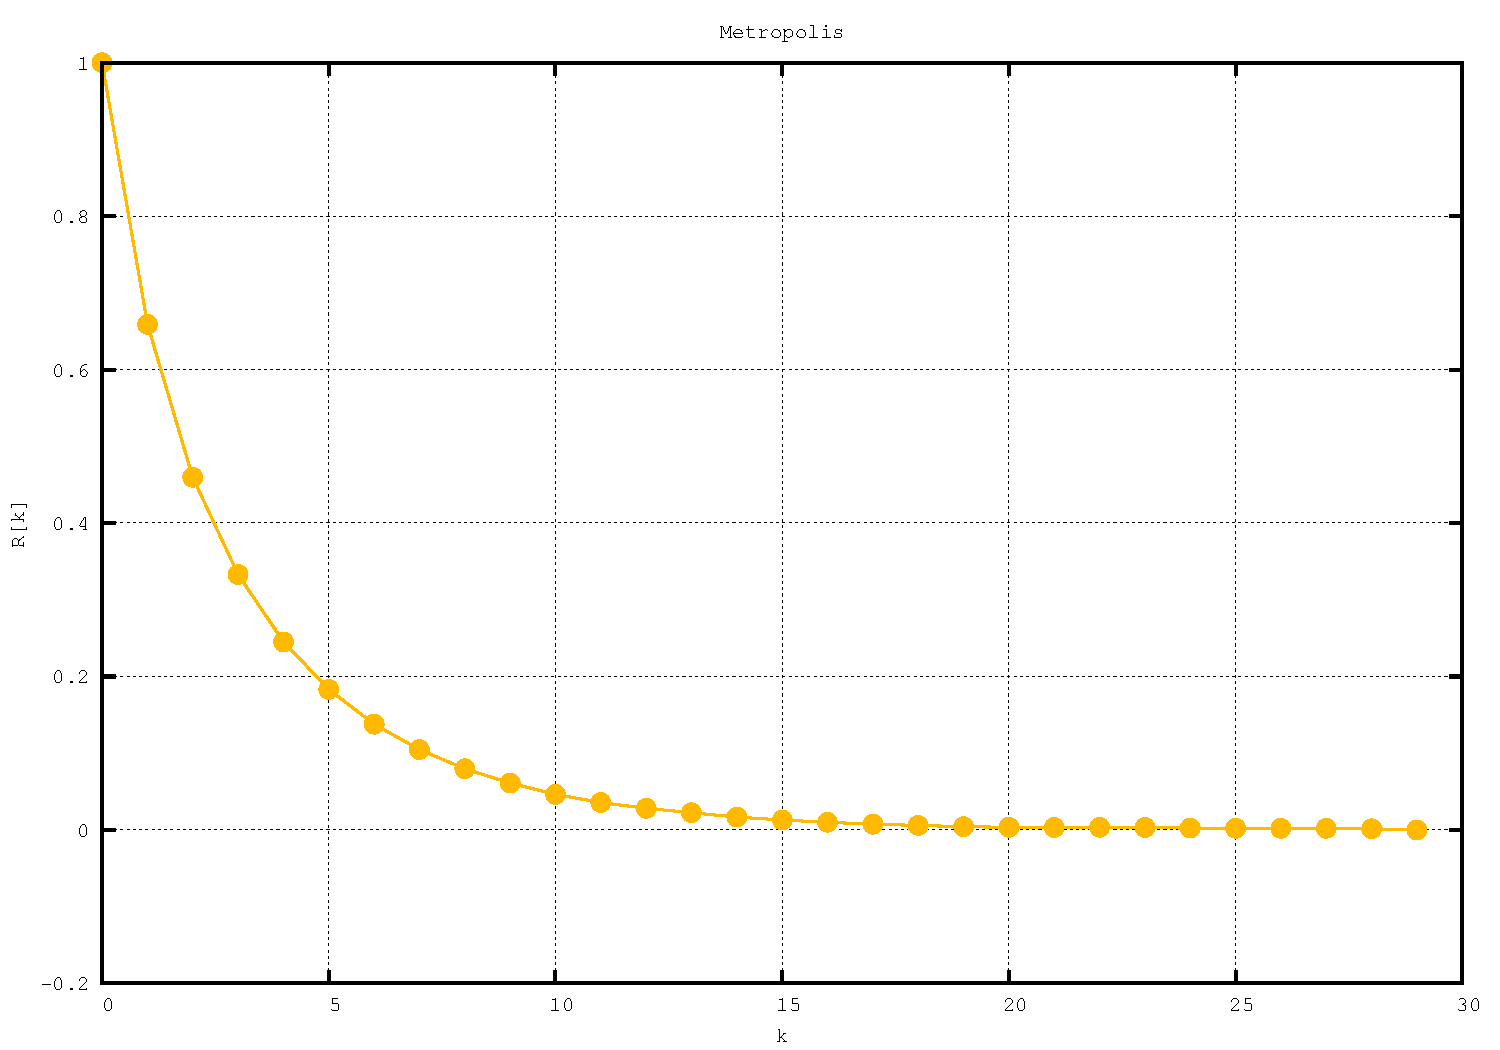
\includegraphics[width=\textwidth]{autocorrelation}
\caption{Autocorrelazione}
\label{fig:autocorrelation}
\end{figure}

\begin{figure}[h]
\centering
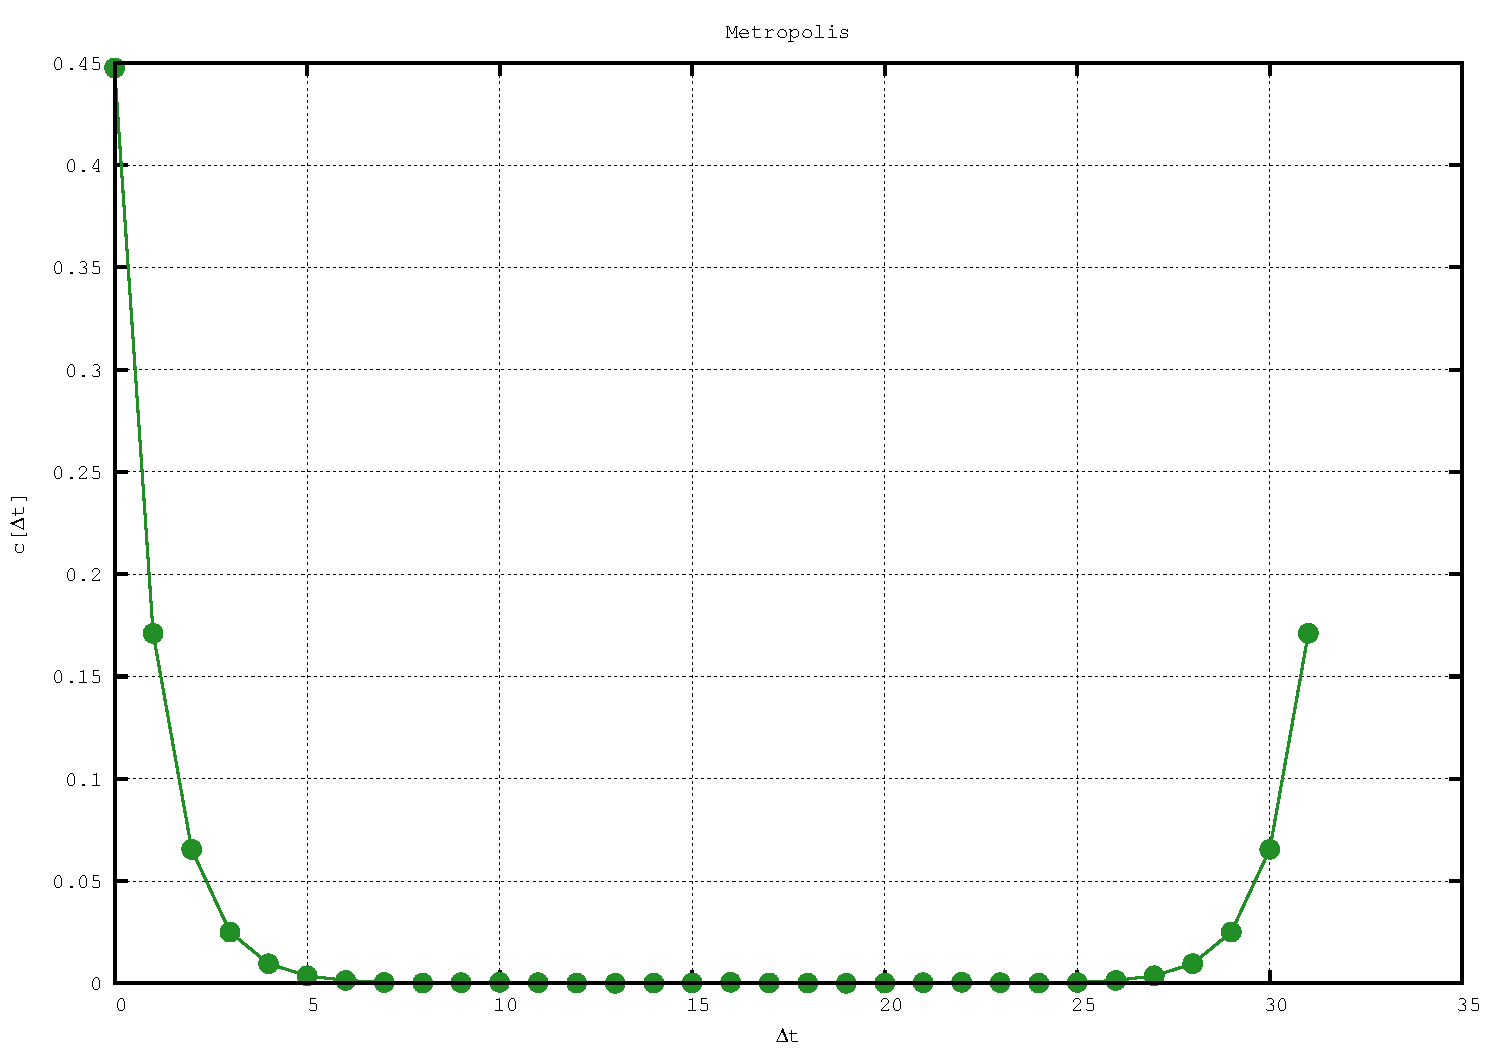
\includegraphics[width=\textwidth]{correlation}
\caption{Correlazione}
\label{fig:correlation}
\end{figure}

\begin{figure}[h]
\centering
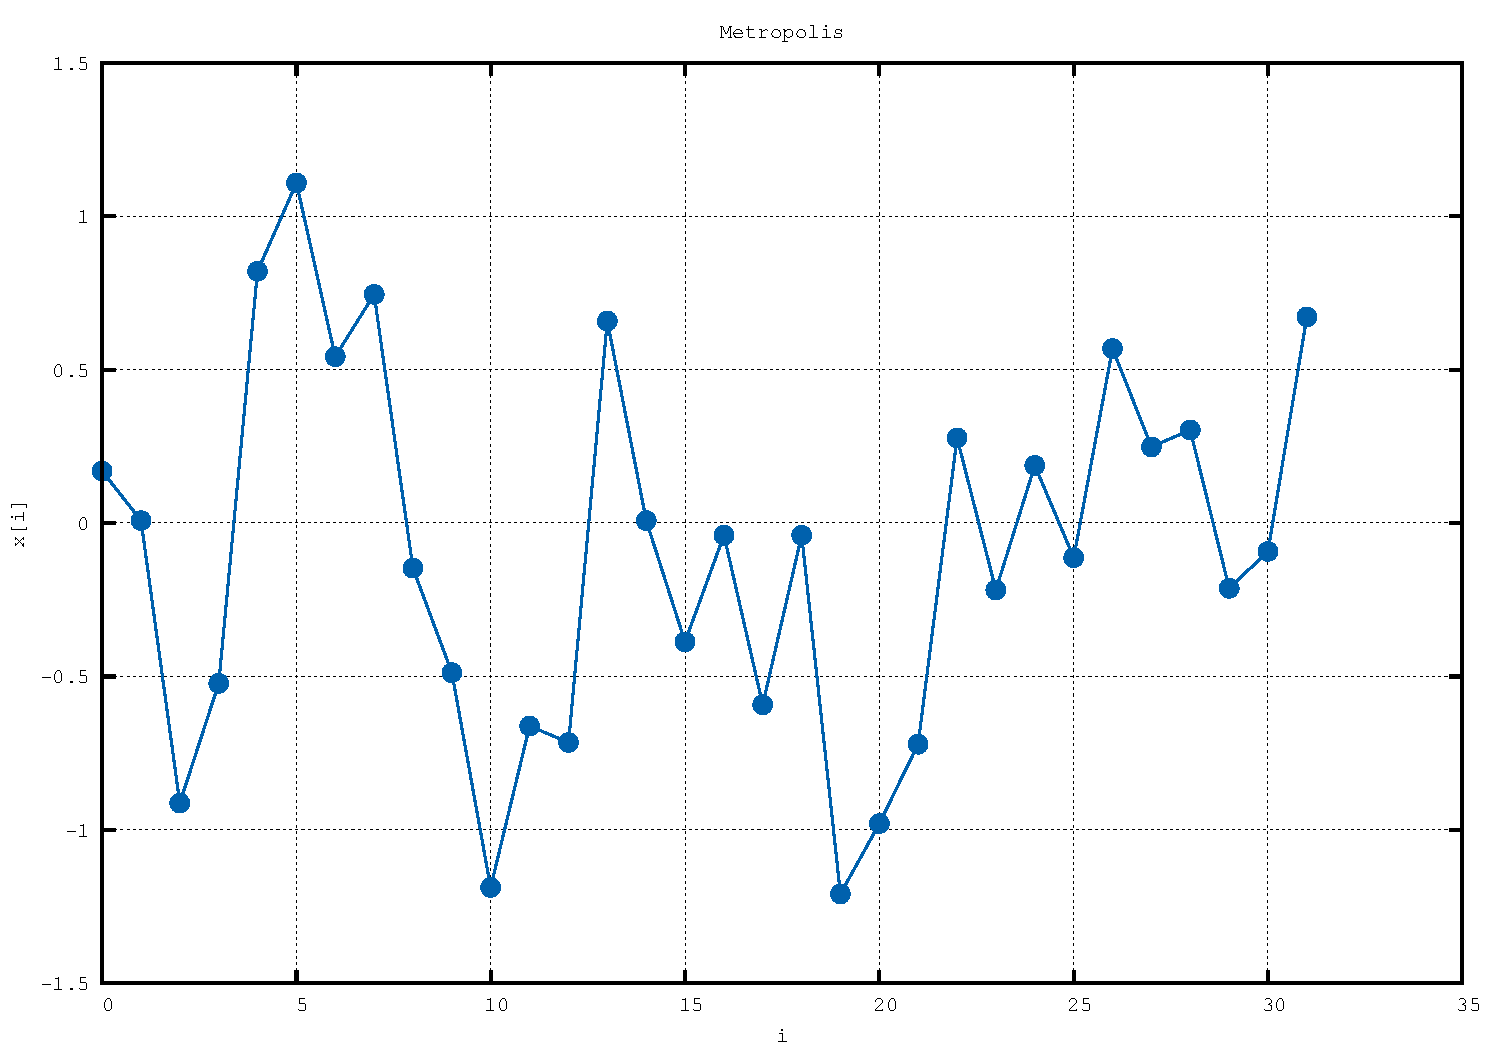
\includegraphics[width=\textwidth]{configuration}
\caption{Configurazione}
\label{fig:configuration}
\end{figure}

\begin{figure}[h]
\centering
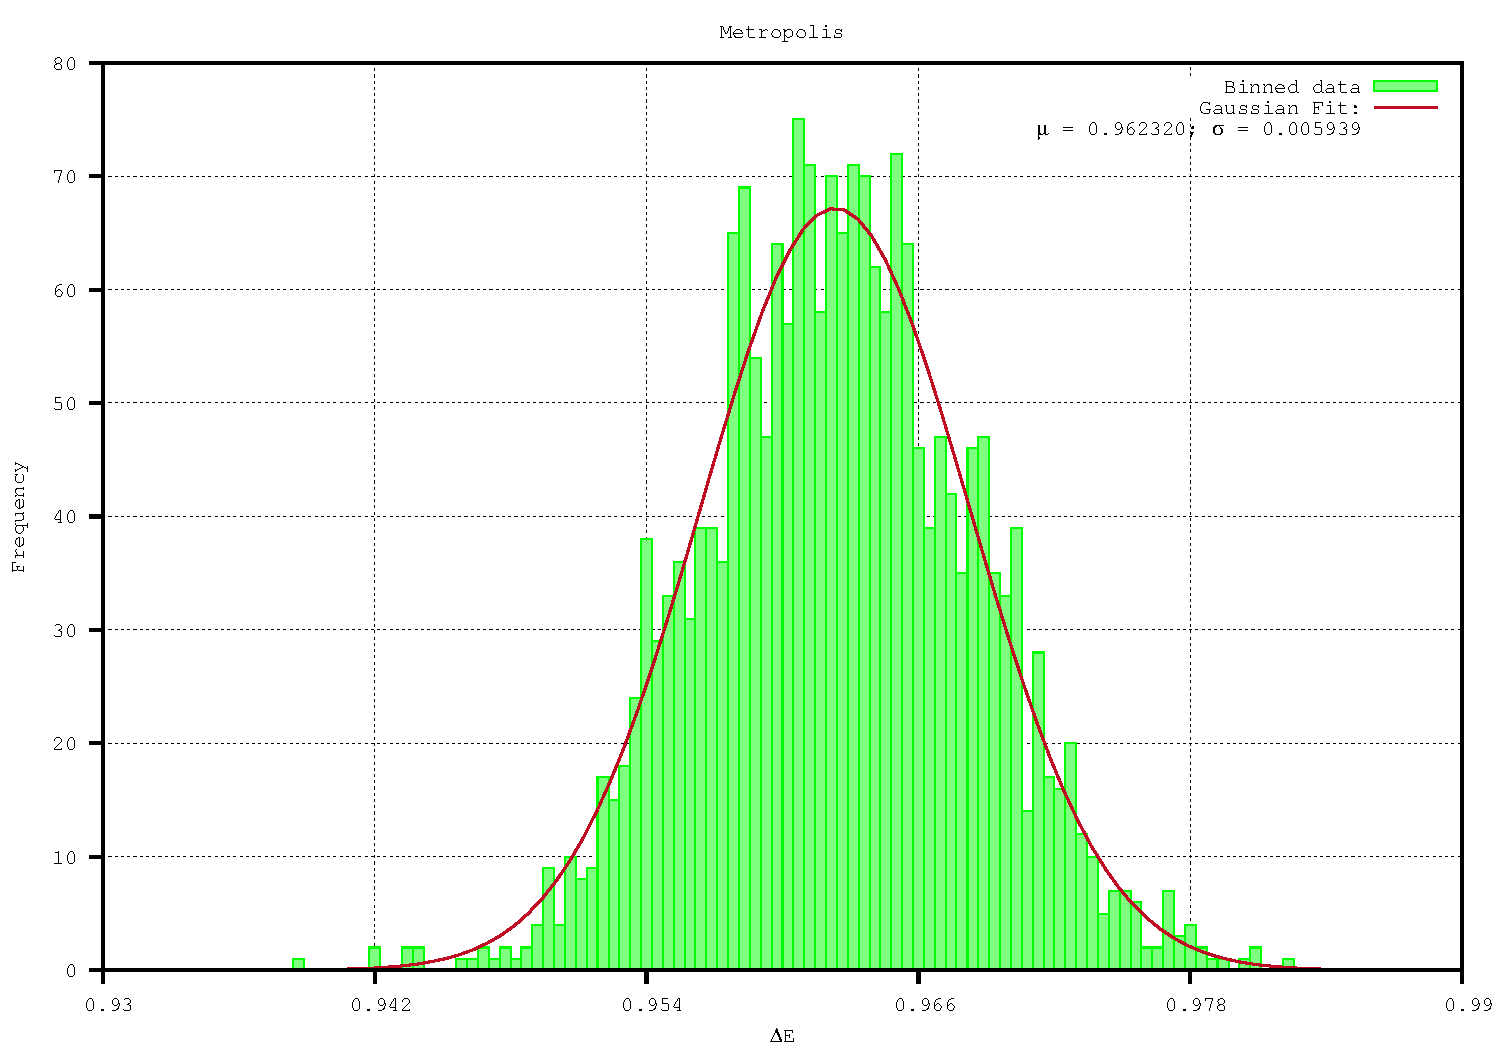
\includegraphics[width=\textwidth]{histogram}
\caption{Istogramma}
\label{fig:histogram}
\end{figure}

\section{Autocorrelazione}
\section{Correlazione}
\section{Calcolo di $\Delta$E}
\section{Calcolo dell'Elemento di Matrice}

\chapter{\huge Metodo Runge-Kutta per Equazioni Differenziali Ordinare}

\section{Il Pendolo Caotico}
\section{Oscillatore di Van Der Pol}
\section{Attrattore di Lorenz}
\section{N-Body Simulation}

\chapter{\huge Altri Metodi per PDE}

\section{Equazioni delle Onde e della Diffusione}
\section{Metodo Implicito ed Equazione di Schr\"{o}dinger}

\end{document}
